%%%%%%%%%%%%%%%%%%%%%%%%%%%%%%%%%%%%%%%%%%%%%%%%%%%%%%%%%%%%%%%%%%%%%%%%%%%%%%%%
%2345678901234567890123456789012345678901234567890123456789012345678901234567890
%        1         2         3         4         5         6         7         8

\documentclass[letterpaper, 10 pt, conference]{ieeeconf}  % Comment this line out if you need a4paper

%\documentclass[a4paper, 10pt, conference]{ieeeconf}      % Use this line for a4 paper

\IEEEoverridecommandlockouts                              % This command is only needed if 
                                                          % you want to use the \thanks command

\overrideIEEEmargins                                      % Needed to meet printer requirements.

% See the \addtolength command later in the file to balance the column lengths
% on the last page of the document

% The following packages can be found on http:\\www.ctan.org
%\usepackage{graphics} % for pdf, bitmapped graphics files
%\usepackage{epsfig} % for postscript graphics files
%\usepackage{mathptmx} % assumes new font selection scheme installed
%\usepackage{times} % assumes new font selection scheme installed
\usepackage{amsmath} % assumes amsmath package installed
\usepackage{amssymb}  % assumes amsmath package installed

\usepackage{color}
\usepackage{graphicx}
\usepackage{subfig}

\newcommand{\comment}[1]{\textcolor{red}{#1}}
%\newcommand{\Mission}[1]{\textbf{\texttt{M#1}}}
\newcommand{\Mission}[1]{\texttt{M#1}}
\newcommand{\Object}{Obj}
\newcommand{\Class}{c}
\newcommand{\ProbObject}{P(\Object)}
\newcommand{\ProbClass}{P(\Class)}

\newcommand{\TrailRegion}{R^{trail}}
\newcommand{\TrailWidth}{w}
\newcommand{\TrailCurvature}{\kappa}
\newcommand{\TrailDMin}{d_{\min}}
\newcommand{\TrailDMax}{d_{\max}}
\newcommand{\TrailLatOffset}{\Delta x}
\newcommand{\TrailHeading}{\theta}
\newcommand{\TrailState}{\mathbf{X}}
\newcommand{\CondProb}[2]{p(#1 | #2)}  % p(Xt|Xt−1)
\newcommand{\TrailLikelihood}{L}
\newcommand{\TrailLikelihoodAppearance}{\TrailLikelihood_{appear}}
\newcommand{\ChiSquared}{\chi^{2}}
\newcommand{\TrailRegionRight}{\TrailRegion_{L}}
\newcommand{\TrailRegionLeft}{\TrailRegion_{R}}
% all of the T sets are train/val
\newcommand{\TrailAnnotatedSet}{\mathtt{trainval}_{trail}}
\newcommand{\TrailBadAnnotatedSet}{\mathtt{trainval}_{bad\_trail}}
%\newcommand{\TrailSeqAnnotatedSet}{\mathcal{A}^{\ast}_{trail}}
\newcommand{\TrailSeqAnnotatedSet}{\mathtt{trainval}_{trail-30}}
\newcommand{\TreeAnnotatedSet}{\mathtt{trainval}_{tree}}

\newcommand{\TrailQualityNet}{\mathtt{D19}_{bad\_trail}}
%\newcommand{\TrailOneDMaskNet}{\mathtt{D19}_{1D\_masks}}
\newcommand{\TrailOneDMaskNet}{\mathtt{D19}_{\mathit{1D\_masks}}}
\newcommand{\TrailRegressionNet}{\mathtt{D19}_{\mathit{regression}}}
%\newcommand{\BoldTrailOneDMaskNet}{\mathtt{D19}_{\mathit{1D\_masks}}}
%\newcommand{\BoldTrailRegressionNet}{\mathtt{D19}_{\mathit{regression}}}
\newcommand{\TrailTwoDMaskNet}{\mathtt{D19}_{2D\_mask}}

% all of the TE sets are test
\newcommand{\TrailTestAnnotatedSet}{\mathtt{test}_{trail}}
\newcommand{\TrailTestBadAnnotatedSet}{\mathtt{test}_{bad\_trail}}

\newcommand{\TrailNearDepth}{d_{near}}
\newcommand{\TrailFarDepth}{d_{far}}
\newcommand{\TrailNearLine}{y_{near}}
\newcommand{\TrailFarLine}{y_{far}}

\title{\LARGE \bf
Deep Learning for Trail Scene Understanding
}


\author{Christopher Rasmussen$^{1}$% <-this % stops a space
%\thanks{*This work was not supported by any organization}% <-this % stops a space
\thanks{$^{1}$Dept. Computer \& Information Sciences,
        University of Delaware, Newark, DE USA
        {\tt\small cer@cis.udel.edu}}%
%\thanks{$^{2}$Bernard D. Researcheris with the Department of Electrical Engineering, Wright State University,
%        Dayton, OH 45435, USA
%        {\tt\small b.d.researcher@ieee.org}}%
}


\begin{document}
\graphicspath{{images/}}

\maketitle
\thispagestyle{empty}
\pagestyle{empty}

%%%%%%%%%%%%%%%%%%%%%%%%%%%%%%%%%%%%%%%%%%%%%%%%%%%%%%%%%%%%%%%%%%%%%%%%%%%%%%%%
\begin{abstract}

  deep learning for trail segmentation and tracking.  semantic understanding of trees
 visually, obviating ladar.  something quantitative about performance increase 
\end{abstract}


%%%%%%%%%%%%%%%%%%%%%%%%%%%%%%%%%%%%%%%%%%%%%%%%%%%%%%%%%%%%%%%%%%%%%%%%%%%%%%%%
%%%%%%%%%%%%%%%%%%%%%%%%%%%%%%%%%%%%%%%%%%%%%%%%%%%%%%%%%%%%%%%%%%%%%%%%%%%%%%%%

\section{INTRODUCTION}

\textit{Scene understanding} is a high-level task in computer vision
that is generally taken to mean semantic labeling of every known part of an
image (or point cloud, in 3-D).  This can take place at a point or pixel level (e.g., \textit{these}
pixels belong to the road, and \textit{those} pixels belong to the
sky) \comment{semantic understanding cites}, or at the level of
discrete object detection \comment{detection cites, including some 3-D}, where bounding
boxes are put around instances of cars, people, sofas, mynah birds, or
whatever else is of interest.

Selection of the set of possible pixel/point categories or object classes,
and constraints on their locations, shapes, and arrangements,
constitutes another level of scene understanding.  Expectations for
the kinds and frequencies of objects to be found in scenes of urban
driving vs. domestic kitchens vs. factory assembly lines will
obviously differ.  Thus prior knowledge of scene type at some level is
valuable for improving labeling/detection performance \comment{cites of scene classification}.  Beyond this,
for robot tasks typically only a subset of \textit{expected} objects
are \textit{relevant}, and so the perception task can be further
narrowed.  Unloading the dishwasher, for example, does not require an
ability to detect toasters or bananas, even though both of
these may be found in the kitchen.

Here we study the problem of \textit{trail following} in the context
of scene understanding.  Driving \comment{cite me} or flying
\comment{cite} along hiking trails or other rough paths in varied
terrain requires, at a minimum, discrimination of the trail region
from the background as shown in a typical scene in
Fig.~\ref{fig:raw_trail}.  Corollary tasks include detection of other
objects that might be found along trails such as signs, hazards like rocks and logs, flora and fauna of interest, and people \comment{cite trail paper that does this}--whether simply as obstacles or as individuals to recognize and interact with.

%%%%%%%%%%%%%%%%%%%%%%%%%%%%%%%%%%%%%%%%%%%%%%%%%%%%%%%%%%%%%%%%%%%%%%%%%%%%%%%%

\begin{figure}[!t]
\captionsetup[subfigure]{labelformat=empty}
\subfloat[]{%
  \centering{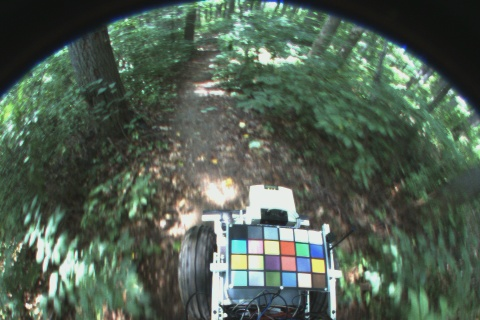
\includegraphics[width=1.0\columnwidth]{000738.jpg}}}\\
\caption{Omnidirectional forest trail image captured from robot.}
\label{fig:raw_trail}
\end{figure}

%%%%%%%%%%%%%%%%%%%%%%%%%%%%%%%%%%%%%%%%%%%%%%%%%%%%%%%%%%%%%%%%%%%%%%%%%%%%%%%%

Classical robot motion planning for navigation and interaction
necessitates the inference of 3-D metric information about scene
components.  This is not strictly necessary--there has been much recent work
on learning to directly map sensor inputs to robot actions without explicit 3-D
representations of the scene \comment{cites}.

\comment{i want to talk about parametric vs. non-parametric
  representation of trail shape.  other deep learning trail following papers don't
  do explicit trail shape at all -- they just go straight from images
  to actions.  pros and cons of various approaches?}

\comment{Working in vehicle coordinates is advantageous
  because... However, given a polygon in the image, we can invert the
  projection and infer the extent of the region in vehicle
  coordinates.}

Rather than attempt to label every trail pixel non-parametrically
\`a la semantic segmentation \comment{cites}, we want to
directly fit a low-dimensional shape to the trail region
immediately in front of the robot.
Geometric constraints on the segmentation improve accuracy
\comment{general cites supporting this?}  and facilitate
frame-to-frame tracking, and trail geometry in the vehicle frame is
needed for motion planning that considers trail edges and in-trail and
nearby obstacles jointly \cite{<FSR2012>}.

\comment{as far as \textit{how} we do this, big obvious point is to
  learn (which of course is what the other trail following papers did,
  albeit in a different fashion) rather than use hand-designed
  objective function.  also want to say something about importance of tracking}

\comment{while we don't attempt to recognize what kind of scene the
  robot is looking at from some large set, we do think that it's
  important to know if a segmentable trail is present or not in the
  image.  so we talk about classifying the image in this way as a
  pre-processing step.}

The robot needs to know if the trail image is bad so that at a minimum
it can switch to a different driving mode, such as stopping and
searching to acquire (or reacquire) the trail.  A secondary goal is to
have a sliding confidence score which guides the robot to slow down or
speed up, or to add or drop cues/sensors as necessary.

% $\TrailRegion$


%Sensor intrinsics and extrinsics are of course required
%for this

\comment{second big point of the paper: the importance of trees.
  tell a little story... problem with how we treat obstacles -- lower density
  vs. collision-free paths with ladar.  small trees violate this: they
  are not many ladar hit points, but they are solid.  so we really need to spot them}

\comment{lay out rest of paper}


%%%%%%%%%%%%%%%%%%%%%%%%%%%%%%%%%%%%%%%%%%%%%%%%%%%%%%%%%%%%%%%%%%%%%%%%%%%%%%%%
%%%%%%%%%%%%%%%%%%%%%%%%%%%%%%%%%%%%%%%%%%%%%%%%%%%%%%%%%%%%%%%%%%%%%%%%%%%%%%%%

\section{BACKGROUND}


%%%%%%%%%%%%%%%%%%%%%%%%%%%%%%%%%%%%%%%%%%%%%%%%%%%%%%%%%%%%%%%%%%%%%%%%%%%%%%%%

\subsection{Trail Following}

\comment{Previous trail following paper that uses learning \cite{<GiustiTrail>}.  Do they have data?  How do they quantify performance?  They trained a 3-category classifier related to heading: facing center (aligned with the trail), facing left, or facing right.  no tracking there, by the way, i believe--every image is analyzed independently}

\comment{IROS 2017 paper from Nvidia \cite{<NvidiaTrail>}.  They use
  YOLO for person detection, DSO for visual odometry and sparse
  obstacle detection, and a multi-head neural network with two
  3-category classifiers: the 3 headings, plus 3 lateral offsets,
  which they say is necessary for the MAV to actually
  work. Performance quantified by classification accuracy and length
  of autonomy}

\comment{my stuff \cite{<FSR2012>}, \cite{<Rasmussen2010>}}

%\comment{this could use a nice diagram.  cite FSR paper/talk about
%  what system could do with robot--not just perception}

%\comment{moved stuff about trail state to datasets, because it seemed
%  like a good place to talk about it.  at least mention the notion of
%  extracting a full region and then doing motion planning on that,
%  which is different from the motion directions inferred by the other
%  two papers I cite, which is sort of a direct mapping from image to
%  robot action.  }

Under the assumption that a unique trail is present in each image, it
is segmented in a top-down, maximum likelihood fashion: multiple
candidate regions are hypothesized and scored using a \textit{trail
  likelihood} function $\TrailLikelihood$, and the highest-scoring
region is the winner.  \cite{<Rasmussen2009>,<Rasmussen2010>} describe
a technique for computing the color appearance likelihood of a
candidate region $\TrailLikelihoodAppearance(\TrailRegion)$ based on
the assumption that the trail region has a strong color and/or
intensity contrast with the left and right neighboring regions
$\TrailRegionLeft$ and $\TrailRegionRight$.  Following
\cite{<Blas2008>}, a small set of exemplar colors for each image was
computed using $k$-means clustering in CIE-Lab space and assign every
pixel one of these $k$ labels. A label histogram is computed for each
candidate region and its neighbors, and the likelihood is obtained as
a weighted combination of contrast and homogeneity (the entropy of the
region color distribution). In \cite{<Rasmussen2010>} the color contrast is
measured by the $\ChiSquared$ distance between the region and its
neighbors. \comment{maybe reproduce formula?}

In \cite{<Rasmussen2010>}, this region was represented in vehicle
coordinates as a constant-width $\TrailWidth$ arc of a circle with
curvature $\TrailCurvature$ over a fixed depth range $[\TrailDMin,
  \TrailDMax]$. The position of the robot with respect to the trail is
given by its lateral offset $\TrailLatOffset$ from the trail
centerline and the difference $\TrailHeading$ between its heading
angle and the tangent to the trail arc. Grouping these yields the
\textit{trail state} vector $\TrailState = (\TrailWidth,
\TrailCurvature, \TrailLatOffset, \TrailHeading)$.  The trail region
is approximated as a polygon which with camera intrinsics and
extrinsics can be projected to the image.

Trail-following entails tracking the trail region over an image
sequence, so \cite{<Rasmussen2010>} used a particle filter
\cite{<ActiveContours>} to incorporate a prior
$\CondProb{\TrailState}{\TrailState_{t-1}}$ on the hypotheses which
keeps them near the predicted location of the trail in the current
frame as derived from the robot’s dynamics, as well as setting
absolute limits on every state parameter.

%%%%%%%%%%%%%%%%%%%%%%%%%%%%%%%%%%%%%%%%%%%%%%%%%%%%%%%%%%%%%%%%%%%%%%%%%%%%%%%%

\subsection{Deep Learning for Detection}

Early CNN-based object detectors operated either in a sliding window
fashion \cite{<Overfeat2014>} or by generating object "proposals"
separately \cite{uijlings2013selective,zitnick2014edge} and then
evaluating these hypotheses. These approaches achieved good results on
difficult detection benchmarks, but were fairly slow and not
well-suited to real-time deployment.  More recently, it has been shown
that CNNs have sufficient power to represent geometric information for
localizing objects, opening the possibility of building
state-of-the-art object detectors that rely exclusively on CNNs free
of proposal generation schemes \cite{<FasterRCNN>,<YOLO>,<YOLO9000>}. In such
approaches, the network is trained end-to-end to predict both the
appearance and geometric information of an object. At test time, given
an input image, the entire network is only evaluated once instead of
at different locations and scales of the image, enabling a
large speed-up.

Redmon \textit{et al.} developed one such unified CNN for real-time
object detection which they called ``You Only Look Once'' (YOLO)
\cite{<YOLO>}. The core idea of YOLO is that it considers the
detection task as a regression problem.  Specifically, the input image
is divided into an $S \times S$ grid of cells, each of which contains
information on $B$ hypothetical object bounding boxes. Each such
bounding box is parametrized by a 5-D vector $[x,y,w,h,\ProbObject]$,
where $\ProbObject=1$ if the center of any ground-truth object
bounding box is inside the cell and $\ProbObject=0$ otherwise.  Each
grid cell also includes a conditional class probability: $\Pr(\Class
\mid \Object)$, where $\Class \in \{C\}$. Accordingly, the
class-specific confidence is given by: $\ProbClass = Pr(\Class \mid
\Object) \ProbObject$.  For each presented image, the output layer of
the network is an $S \times S \times (B * 5 + C)$ tensor.  Non-maximal
suppression is used to remove duplicate detections, followed by
thresholding on $\ProbClass$.

Using values of $S=7$ and $B=2$, YOLO achieved a very high mAP (mean
average precision) on the 20-class PASCAL VOC 2007 \cite{<PASCAL>}
while running at a speed of 45 fps, faster than any comparable system.
One shortcoming of YOLO is its difficulty at detecting small objects
that are very close to each other since it only predicts two bounding
boxes within one class per grid cell.  This is a concern for us since
many trees appear quite thin, occupying a small portion of each image horizontally.

%Compared with other real-time object
%detectors such as the deformable part model approach of \cite{<DPM>},

%And the experiment also
%shows that YOLO gets fewer background errors but more localization
%errors than Fast R-CNN \cite{<FastRCNN>}. Apparently to reduce
%localization errors would be another problem to solve in the further
%works.

%It has been proved that YOLOv2 is faster than most of other
%detection frameworks (e.g. FasterR-CNN, ResNet \cite{<ResNet2016>},
%SSD \cite{<SSD>}).

Recently, Redmon and Farhadi proposed another real-time detection
system, YOLOv2 \cite{<YOLO9000>}, that aims to improve on the
localization and recall performance of YOLO.  Several key
modifications in YOLOv2 include batch normalization on every
convolutional layer to enhance convergence and regularize the model, a
higher input image resolution of $448 \times 448$ and finer grid with $S=13$, and the replacement
of YOLO's fully connected layers which directly regress bounding box
coordinates with an ``anchor box'' concept adapted from
\cite{<FasterRCNN>}.  YOLOv2 uses a new classification model as the
front end which is somewhat similar to VGG models \cite{<VGG2015>}, but with global
average pooling to make predictions and $1 \times 1$ filters to
compress features representations between $3 \times 3$ convolutions.
The classification model is called ``Darknet-19'' and has 19
convolution layers and 5 max-pooling layers.

YOLOv2's mAP on PASCAL VOC 2012 is significantly improved over YOLO and
comparable to current leaders like Faster R-CNN with ResNet
\cite{<ResNet2016>} and SSD512 \cite{<SSD>}, while running from 2 to
10 times faster.

%%%%%%%%%%%%%%%%%%%%%%%%%%%%%%%%%%%%%%%%%%%%%%%%%%%%%%%%%%%%%%%%%%%%%%%%%%%%%%%%

\subsection{Deep Learning for Tracking}

\comment{Cropping approach for smoothness, no explicit motion model \cite{<100FPSTracking>}}

%%%%%%%%%%%%%%%%%%%%%%%%%%%%%%%%%%%%%%%%%%%%%%%%%%%%%%%%%%%%%%%%%%%%%%%%%%%%%%%%
%%%%%%%%%%%%%%%%%%%%%%%%%%%%%%%%%%%%%%%%%%%%%%%%%%%%%%%%%%%%%%%%%%%%%%%%%%%%%%%%

\section{DATASETS}

%%%%%%%%%%%%%%%%%%%%%%%%%%%%%%%%%%%%%%%%%%%%%%%%%%%%%%%%%%%%%%%%%%%%%%%%%%%%%%%%

%, shown in \comment{Fig.~\ref{fig:warthog}}

Trail and tree image data were collected from a single color camera
with an omnidirectional lens, mounted in a downward-pointing
configuration on a Segway RMP 400 four-wheeled robot.  This
arrangement allows 360-degree visibility of the terrain around the
robot and obstacles up to a height of about 1.5 m.  We assume the
robot does not reverse, so only half of the full image ($480 \times 320$ pixels) is used as
shown in Fig.~\ref{fig:raw_trail}.  
  
%,

%\comment{photo if there's space?}

%%%%%%%%%%%%%%%%%%%%%%%%%%%%%%%%%%%%%%%%%%%%%%%%%%%%%%%%%%%%%%%%%%%%%%%%%%%%%%%%

%\begin{figure}[!t]
%%\captionsetup[subfigure]{labelformat=empty}
%\subfloat[]{%
%  \centering{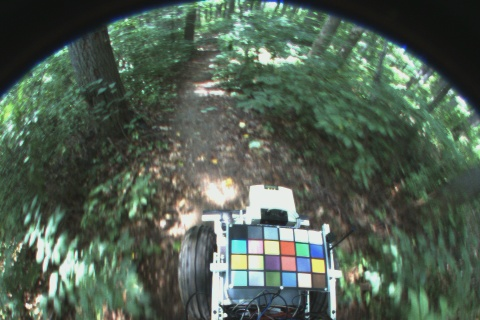
\includegraphics[width=1.0\columnwidth]{000738.jpg}}}\\
%\subfloat[]{%
%  \centering{\includegraphics[width=1.0\columnwidth]{crop_overlay_no_lines_Aug_05_2011_Fri_12_29_30_PM_omni_images_%000738.png}}}
%\caption{(a) Forest trail image captured from robot; (b) Detail of image with trail segmentation ROI (inner gray re%ctangle), ground truth trail region (green polygon), tree search ROI (outer gray rectangle), and ground truth tree %bounding boxes (yellow rectangles) overlaid.}
%\label{fig:trail_explainer}
%\end{figure}

\begin{figure}[!t]
\captionsetup[subfigure]{labelformat=empty}
\subfloat[]{%
  \centering{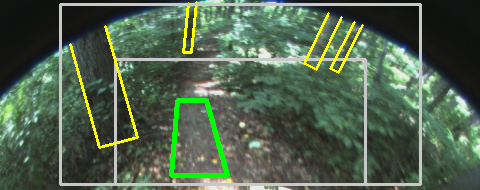
\includegraphics[width=1.0\columnwidth]{crop_overlay_no_lines_Aug_05_2011_Fri_12_29_30_PM_omni_images_000738.png}}}
\caption{Detail of image in Fig.~\ref{fig:raw_trail} with trail segmentation ROI (inner gray rectangle), ground truth trail region (green quadrilateral), tree search ROI (outer gray rectangle), and ground truth tree oriented bounding boxes (yellow rectangles) overlaid.}
\label{fig:trail_explainer}
\end{figure}

%%%%%%%%%%%%%%%%%%%%%%%%%%%%%%%%%%%%%%%%%%%%%%%%%%%%%%%%%%%%%%%%%%%%%%%%%%%%%%%%

%Nonetheless, here we only use the portion of the image in front
%of the robot

%\comment{camera intrinsics and extrinsics are known but not necessarily used.  need to show ROIs}


%%%%%%%%%%%%%%%%%%%%%%%%%%%%%%%%%%%%%%%%%%%%%%%%%%%%%%%%%%%%%%%%%%%%%%%%%%%%%%%%

\subsection{Trail shape, quality}
\label{sec:trail}

We assume camera intrinsics and extrinsics relative to the robot are
known. In \cite{<FSR2012>} this information was used to mask out the
black regions in the upper corners of the image and the robot itself
for image processing.  Here we simply reduce the image to a $250
\times 125$ region of interest, the \textit{trail ROI}, as indicated
by the inner gray rectangle in Fig.~\ref{fig:trail_explainer}.  This
excludes the black areas, robot, and more distant parts of the ground
plane (beyond roughly 5 m), but is wide enough to keep the left and
right edges of the trail region visible through most (but not all)
variations in trail shape and robot maneuvers.

For annotation purposes, the region of the trail just in front of the
robot is approximated by a quadrilateral constrained to have its near
and far edges at fixed distances $\TrailNearDepth, \TrailFarDepth$ (here about 1 m and
2.5 m) along the nominal ground plane in front of the robot.  The
image projection of this quadrilateral, exemplified by the green shape
in Fig.~\ref{fig:trail_explainer}, thus has horizontal bottom and top
edges in the trail ROI at $\TrailNearLine$ and $\TrailFarLine$ (ignoring radial
distortion from the lens).  These lines are shown in blue and red
respectively in Fig.~\ref{fig:nearfar_explainer}.  The intersections
of the left $L$ and right $R$ trail boundaries with $\TrailNearLine$ and
$\TrailFarLine$ define the trail quadrilateral with 4 variables:
$(x^{L}_{far}, x^{R}_{far}, x^{L}_{near}, x^{R}_{near})$.

Figs.~\ref{fig:nearfar_explainer}(a-f) show several samples of ground truth for the
quadrilateral trail region approximation in different terrain and
lighting conditions.  Figs.~\ref{fig:nearfar_explainer}(g-l) are
examples of images which were annotated as \textit{bad trail}, or not
containing a complete or suitable trail region.  In
Fig.~\ref{fig:nearfar_explainer}(g) the robot is in a parking lot,
approaching the trailhead, but there is no trail region yet between
$y_{near}$ and $y_{far}$.  In Fig.~\ref{fig:nearfar_explainer}(h) the
robot is pointing off the trail and only sees an empty field.  In
Fig.~\ref{fig:nearfar_explainer}(i) the left side of the trail is not
completely in the trail ROI because of the robot orientation and width of the trail, and similarly in
Fig.~\ref{fig:nearfar_explainer}(j) only a portion of the trail is
visible at left.  In Figs.~\ref{fig:nearfar_explainer}(k) and (l) the
trail is completely visible, but in the former case it curves so
sharply that it does not intersect $y_{far}$, and in the latter case
the branching makes a quadrilateral approximation too poor.

For the most part, over the chosen depth range our linear approximation to the trail
shape and an assumption that the ground is planar are reasonable.
Thus, we can invert the camera projection
and obtain the trail region in vehicle coordinates.  These variables
then allow the calculation of variables relevant to motion planning
such as trail width, lateral offet, and heading.  Trail curvature, however, must
be estimated with temporal filtering.


%\comment{This may occur because the trail's width and lateral offset caused
%one side to be outside the trail ROI, the trail's heading and
%curvature were such that it did not intersect the far line, or there
%was a branch that made the shape assumption an especially poor fit.}

%maybe mention previous/smaller dataset with curved borders}


%we investigate whether the image can be reduced to an even

%allow common variations in trail lateral offset,
%heading, and width while still

%\comment{Here we focus on the segmentation of the trail region in the image. For simplicity ...}

%we crop it to the \comment{some color} rectangle

%\comment{how full image was cropped to not include robot, see fairly far ahead and left/right, then resized.}


%%%%%%%%%%%%%%%%%%%%%%%%%%%%%%%%%%%%%%%%%%%%%%%%%%%%%%%%%%%%%%%%%%%%%%%%%%%%%%%%
% good
% 000006  bridge
% 000011, 000076, 000138, 000248  shadow mixed
% 000111, 000215  skinny tree to left
% 000125  field, skinny trail almost off image left
% 000179  coming to branch

% bad
% *404 parking lot transition to trail
% 407, 417, *512 too much curve
% *408 off trail in grass
% 423, *461 tree blocking, trail to left
% 439, 453, 504, *753 too wide
% 532, 752, *773 strange shape

% 414, 427, 466, 485, 558, 573, 632, 741, 821 should not be in bad set

\begin{figure}[!t]
%\captionsetup[subfigure]{labelformat=empty}
\centering{\subfloat[]{%
    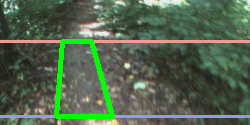
\includegraphics[width=0.32\columnwidth]{000343_trail_roi_good.png}}
 \hspace{0.001\in}
\subfloat[]{%
  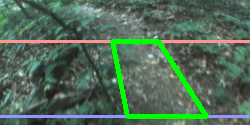
\includegraphics[width=0.32\columnwidth]{000215_trail_roi_good.png}}
 \hspace{0.001\in}
\subfloat[]{%
  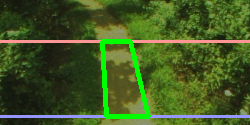
\includegraphics[width=0.32\columnwidth]{000076_trail_roi_good.png}}}\\
\vspace{-0.06in}
\centering{\subfloat[]{%
    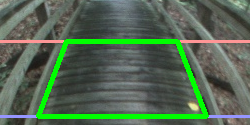
\includegraphics[width=0.32\columnwidth]{000006_trail_roi_good.png}}
%    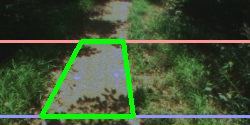
\includegraphics[width=0.32\columnwidth]{000138_trail_roi_good.png}}
 \hspace{0.001\in}
\subfloat[]{%
  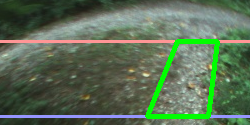
\includegraphics[width=0.32\columnwidth]{000179_trail_roi_good.png}}
 \hspace{0.001\in}
\subfloat[]{%
  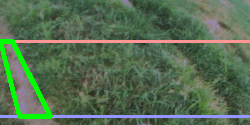
\includegraphics[width=0.32\columnwidth]{000125_trail_roi_good.png}}}\\
\centering{\subfloat[]{%
    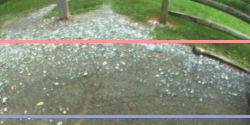
\includegraphics[width=0.32\columnwidth]{000404_trail_roi_bad.png}}
 \hspace{0.001\in}
\subfloat[]{%
  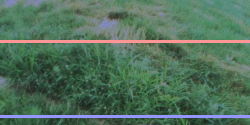
\includegraphics[width=0.32\columnwidth]{000408_trail_roi_bad.png}}
 \hspace{0.001\in}
\subfloat[]{%
  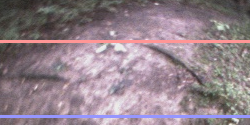
\includegraphics[width=0.32\columnwidth]{000753_trail_roi_bad.png}}}\\
\vspace{-0.06in}
\centering{\subfloat[]{%
    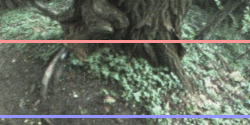
\includegraphics[width=0.32\columnwidth]{000461_trail_roi_bad.png}}
 \hspace{0.001\in}
\subfloat[]{%
  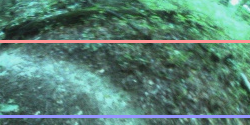
\includegraphics[width=0.32\columnwidth]{000512_trail_roi_bad.png}}
 \hspace{0.001\in}
\subfloat[]{%
  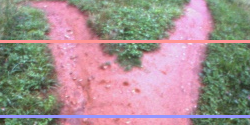
\includegraphics[width=0.32\columnwidth]{000773_trail_roi_bad.png}}}
\caption{(a-f) Sample of trail ROIs with overlays of ground truth trail region quadrilaterals in green and $\TrailNearLine / \TrailFarLine$ lines in blue/red.  The source of image (a) is the same as Figs.~\ref{fig:raw_trail} and \ref{fig:trail_explainer}.  (g-l) Sample of trail ROIs from $\TrailBadAnnotatedSet$.  In these images, a \textit{good} trail region either is not completely visible within the image or does not extend over the entire search depth range.}
\label{fig:nearfar_explainer}
\end{figure}

%%%%%%%%%%%%%%%%%%%%%%%%%%%%%%%%%%%%%%%%%%%%%%%%%%%%%%%%%%%%%%%%%%%%%%%%%%%%%%%%

%\comment{add fig with 4 explainer images showing the near/far lines + GT in the trail ROI only for (1) the image we already have, (2) another area...maybe mixed with strong shadows but good geometry, (3) bad field because trail just partially in trail ROI (hence no GT), and (4) bad forest because trail curves too much (hence no GT).
%\comment{Use POT display to figure out how far away in vehicle coords near and far lines are, approximately}

%\comment{Far/near = red and blue horizontal lines -- separate image?}

%\comment{by this definition, the trail was not always visible.  if the robot left the trail, or it curved enough, one or both of the far/near lines would not intersect with a trail.  These were marked as ``no trail'' images.}

%%%%%%%%%%%%%%%%%%%%%%%%%%%%%%%%%%%%%%%%%%%%%%%%%%%%%%%%%%%%%%%%%%%%%%%%%%%%%%%%

\subsection{Trees}

Trees occur next to the trail, so of necessity the \textit{tree ROI} is
wider than the trail ROI.  In order to detect more distant trees, and
to include pixels higher up the trunk for more confident
identification, the search area is also extended upwards.  The full
extent of the $360 \times 180$ tree ROI can be seen in the outer gray rectangle in Fig.~\ref{fig:trail_explainer}.

%This area does include some of the black portions of the image

%\comment{relationship to trail images -- larger crop rectangle is the \textit{tree ROI} --
%  maybe one summary omni image that shows trail region with trees
%  marked?}

A tree annotation is essentially a tree trunk bounding box.
Axis-aligned rectangles are standard for detection, but here we make
two important modifications.  First, because of the spherical
distortion of the omnidirectional image, the box is oriented.  Even
though nearly all tree trunks are roughly vertical, depending on where
they are in the image, they will appear to ``lean'' and a standard
bounding box will be a poor fit.  Second, because the tops of trees
are not visible, there is no top to the bounding box.  Therefore each
tree $T$ is parametrized by an oriented rectangle defined by the pixel
position of the bottom center of its trunk (where it meets the
ground), the average pixel width of its trunk, and its image
orientation, or $(x_{T}, y_{T}, w_{T}, \theta_{T})$.

There are many trees in the forest, and we performed several tests in
order to filter out irrelevant or only partially visible trees and to
keep the annotation job tractable.  As with the \textit{bad trail}
images, we exclude any tree $T$ such that either the left or right
edge at its base is outside the tree ROI.  Also, $T$ is ignored if the
fraction of the visible part of the tree in the tree ROI
is too small ($f_{visible}(T) < 0.75$) , or if it is too thin ($w_{T} < 5$
pixels)--this is usually due to distance.

%Because the \textit{raison d'\^etre} for the tree detector is to find
%navigational hazards which are relatively thin and vertical, we also
%included wooden posts found along the trail.  These could stand alone
%with signs attached, or be part of fences or railings (such as the
%bridge in Fig.~\ref{fig:nearfar_explainer}(d)).

%\comment{filter by minimum width, other factors?}

%%%%%%%%%%%%%%%%%%%%%%%%%%%%%%%%%%%%%%%%%%%%%%%%%%%%%%%%%%%%%%%%%%%%%%%%%%%%%%%%

\subsection{Training/validation}

% 82,341 total
% 4,634 bad
% 77,707 good

To create a train/validation dataset, images were selected from multiple
robot runs along a combined hiking/mountain-biking trail in the
eastern U.S. over three days in different summer months and years.
This trail forms a 1.7 km-long loop through varied terrain including
grassy fields, mixtures of dense bushes and shorter trees, and mature
forest with sections of both sparse and dense understory foliage.  The
weather varied from sunny to overcast.  In total, over 82,000 images
were logged at 10 fps from roughly 4.2 km of driving under both manual
and autonomous control (using the approach of \cite{<FSR2012>}).  The
robot speed was typically between 0.75 m/s (autonomous) and 1.5 m/s
(manual), but it sometimes paused for ladar scans or was stopped and
repositioned to begin a new segment.  Just over 4,600 of these images
were marked as \textit{bad trails} as defined above.

\subsubsection{Trail shape} From among the nearly 78,000 \textit{good}
images, a subset of about 2.5\% were selected for quadrilateral trail
shape annotation, randomly but with a separation of at least 40-50
frames to minimize overly similar images.  In all, a set
$\TrailAnnotatedSet$ of 2,018 images containing the complete trail
region were annotated.  A subset $\TrailBadAnnotatedSet$ of 2,711 bad
trail images were randomly selected for training/validation.

To facilitate tracking evaluation and learning
dynamics, each annotated image $I_{t} \in \TrailAnnotatedSet$ at time
$t$ (using frames as units of time) was supplemented with trail
annotations for the preceding 30 frames (roughly 3 seconds).  Only
three of these frames, $I_{t-10}$, $I_{t-20}$, and $I_{t-30}$, were
manually annotated.  Annotations for the remaining frames were derived
from these through cubic interpolation.  This set of
annotated image sequences will be called $\TrailSeqAnnotatedSet$

%\subsubsection{Trail quality} \comment{Composition of good/bad (quality) dataset $\TrailBadAnnotatedSet$.  Basically $\TrailAnnotatedSet$ + random subset of bad images.}

% $I_{f-1}-I_{f-9}$, $I_{f-11}-I_{f-19}$, and $I_{f-21}-I_{f-29}$

\subsubsection{Trees} A 650-image subset $\TreeAnnotatedSet \subset
\TrailAnnotatedSet$ contains at least one tree according to the
filtering criteria previously described.  1,440 trees were
annotated in this set.

%%%%%%%%%%%%%%%%%%%%%%%%%%%%%%%%%%%%%%%%%%%%%%%%%%%%%%%%%%%%%%%%%%%%%%%%%%%%%%%%

\subsection{Testing}

We also created a test set taken in late winter which consisted
of part of the same train/validation trail loop, plus one run each on a paved campus
path and a gravel path at a suburban park.  Visual conditions were
significantly different, with color contrast significantly reduced.
See \comment{winter vs. summer pics} for a comparison of the same
%\comment{Fig.~\ref{fig:wintersummer}} for a comparison of the same
section of trail at different times of year.  The total number of
logged images was 13,179, of which 1,302 were marked as \textit{bad
  trails}.

\subsubsection{Trail shape} Shape annotations were made for about 5\% of good trail images (using 20-frame intervals
from the captured sequences), resulting in a set
$\TrailTestAnnotatedSet$ of 553 images.  Similarly, a
representative set $\TrailTestBadAnnotatedSet$ of 256 bad trail
images was selected.

\subsubsection{Trees} \comment{something to say here?}


%\comment{size of set?
%  maybe another area in summer?}

% i counted 13,180 somewhere, but map_trailGT is reporting 13,179

%\comment{For tree detection, the same dataset as the trail was used, with the same train/test split.  but not all the images had trees -- mention how many this was, and how many trees there were in all}

%%%%%%%%%%%%%%%%%%%%%%%%%%%%%%%%%%%%%%%%%%%%%%%%%%%%%%%%%%%%%%%%%%%%%%%%%%%%%%%%
%%%%%%%%%%%%%%%%%%%%%%%%%%%%%%%%%%%%%%%%%%%%%%%%%%%%%%%%%%%%%%%%%%%%%%%%%%%%%%%%

\section{TRAIL ANALYSIS}

\subsection{Quality}

%As mentioned in the previous section, not all images contain a
%view of the trail that permits it to be fully segmented.

In \cite{<FSR2012>}, bad trail classification was performed by simply
thresholding the likelihood of the trail tracker state, as this
represents the ``quality'' of the current trail estimate.  This
estimate is nominally optimal, so if the tracker cannot find a
high-valued state, the system may infer that there is no clear trail
in the image.

Here, we use the labeled data to train a \textit{trail quality} neural network 2-category
classifier to recognize bad trail images.
Specifically, the color trail ROI is resized to $160 \times 80$ and
input to a resized Darknet-19 convolutional neural network
\cite{<YOLO9000>}, which is used as a feature-finding front end.  This
module terminates with 1,024 $5 \times 2$ feature maps.  This is
followed by a $1 \times 1$ convolutional layer with 2 filters and linear activations.  Each
of the 2 resulting feature maps is average-pooled, then a softmax
function is applied to obtain the final 2-unit output layer.
This network will be called $\TrailQualityNet$.

%When
%this likelihood drops below a threshold, the robot stops and a ladar
%point cloud is gathered for structural analysis.}



%\comment{Darknet-19 two-category classifier: ``good'' and ``bad'' with respect to trail.}

%%%%%%%%%%%%%%%%%%%%%%%%%%%%%%%%%%%%%%%%%%%%%%%%%%%%%%%%%%%%%%%%%%%%%%%%%%%%%%%%

\subsection{Segmentation}

If the quality network classifies an image as containing a good trail,
the robot then tries to estimate the best-fit trail quadrilateral
$(\hat{x}^{L}_{far}, \hat{x}^{R}_{far}, \hat{x}^{L}_{near},
\hat{x}^{R}_{near})$ using a \textit{trail shape} network.  Directly
regressing a bounding box (i.e., outputting coordinates) from an image
is a highly non-linear and difficult-to-learn mapping
\cite{<JointCNN>,<FlowingConvNets>}.  Furthermore, there is the
question of how to enforce $x^{L}_{*} < x^{R}_{*}$.  At the opposite
end of the spectrum, training the network to classify each pixel as
either part of the trail or part of the background may be an easier task, but
underconstrained--and non-trivial post-processing must be done on this
output \textit{trail mask} to obtain the quadrilateral vertices.

Rather, we use an idea similar to
\cite{<FlowingConvNets>}, which labels joint locations in images of
people, and train the network to output a \comment{blah blah
  ``heatmap'', where high-value pixels belong to the trail and
  low-value pixels to the background.}

In \cite{<FlowingConvNets>}, at training time each ground truth joint
position is indicated by a fixed-variance Gaussian (each joint has a
separate heatmap) and the loss is the sum of squared differences.  At
test time, each joint's predicted heatmap is post-processed to obtain
the most likely joint location as the brightest pixel location.  We
want to generalize this to learn \textit{masks} of \comment{trail
  pixels, shown in blah blah heamap fig?}
%Fig.~\ref{fig:heatmap}}.

\comment{more explanation of heatmap/mask concept--cite torr paper for more complex shapes.}
  
Below, we outline several variants along this continuum, all of which
start with the Darknet-19 feature-finding front end 
\cite{<YOLO9000>} used in the trail quality network described above.

\paragraph{$\TrailRegressionNet$} The Darknet-19 terminal feature maps are followed by 2 fully-connected
layers of 1,024 units each, then a fully-connected 4-unit output layer (all with linear activations).
The output layer's units are interpreted directly as the trail quadrilateral vertices
$(\hat{x}^{L}_{far}, \hat{x}^{R}_{far}, \hat{x}^{L}_{near}, \hat{x}^{R}_{near})$.  \comment{loss is just SSE?}

\paragraph{$\TrailOneDMaskNet$} The Darknet-19 terminal feature maps are again followed by 2 fully-connected
layers of 1,024 units each, but now the final fully-connected output
layer has 320 units, and these layers all have ReLU activations.
Consider a \textit{trail mask} image with the same dimensions as the
trail ROI \comment{picture to illustrate?}.  The first 160 units of
the output layer are predictions of the pixels of the trail mask image
along the $\TrailFarLine$ row, and the final 160 units predict the
mask's pixels along $\TrailNearLine$.

\comment{this method is hybrid--heatmap + constraints}

\comment{actual details of thresholding output layer to binarize, then biggest connected component
  with a maximum gap?}

\comment{Ground truth quadrilateral ``rasterized'', rows at $\TrailFarLine, \TrailNearLine$ concatenated to make 320-vector.  Loss is SSE between this and network output}

%In this case the output layer would be the same size as the input layer
%($160 \times 80$)

%Using a simplified version of VGG-16 \cite{<VGG2015>} as the front end,
%we were successful \comment{numbers?}, but various comparisons showed
%that the mask approach works better.


%\comment{used of TensorFlow for some experiments, Darknet for later ones}

%\comment{the trail ROI is scaled down to $160 \times 80$ before being input to the neural network.}


%%%%%%%%%%%%%%%%%%%%%%%%%%%%%%%%%%%%%%%%%%%%%%%%%%%%%%%%%%%%%%%%%%%%%%%%%%%%%%%%

\subsection{Tracking}

\comment{can just use trail regions as observations in Kalman filter or EKF.}

\comment{or do I finally figure out LSTM for heatmap prediction?}

%%%%%%%%%%%%%%%%%%%%%%%%%%%%%%%%%%%%%%%%%%%%%%%%%%%%%%%%%%%%%%%%%%%%%%%%%%%%%%%%
%%%%%%%%%%%%%%%%%%%%%%%%%%%%%%%%%%%%%%%%%%%%%%%%%%%%%%%%%%%%%%%%%%%%%%%%%%%%%%%%

\section{TREE DETECTION}

\comment{we use YOLOv2, modified for oriented bounding boxes.}

\comment{note that \cite{<NvidiaTrail>} used YOLO for person detection along trail, which triggers some particular behavior}

%%%%%%%%%%%%%%%%%%%%%%%%%%%%%%%%%%%%%%%%%%%%%%%%%%%%%%%%%%%%%%%%%%%%%%%%%%%%%%%%

%\begin{figure}[thpb]
%  \centering \framebox{\parbox{3in}{We suggest that you use a text
%      box to insert a graphic (which is ideally a 300 dpi TIFF or
%      EPS file, with all fonts embedded) because, in an document,
%      this method is somewhat more stable than directly inserting
%      a picture.  }}
%  %\includegraphics[scale=1.0]{figurefile}
%  \caption{Inductance of oscillation winding on amorphous
%    magnetic core versus DC bias magnetic field}
%  \label{figurelabel}
%\end{figure}
   
%%%%%%%%%%%%%%%%%%%%%%%%%%%%%%%%%%%%%%%%%%%%%%%%%%%%%%%%%%%%%%%%%%%%%%%%%%%%%%%%

%%%%%%%%%%%%%%%%%%%%%%%%%%%%%%%%%%%%%%%%%%%%%%%%%%%%%%%%%%%%%%%%%%%%%%%%%%%%%%%%
%%%%%%%%%%%%%%%%%%%%%%%%%%%%%%%%%%%%%%%%%%%%%%%%%%%%%%%%%%%%%%%%%%%%%%%%%%%%%%%%

\section{RESULTS}

We used the Darknet-19 library \cite{<Darknet>}, which is GPU-accelerated, for all
neural network training and testing.  All training started from random
weights and used a batch size of 128 images unless otherwise noted.

The images annotated with trail shape $\TrailAnnotatedSet$ were randomly split
80/20 to get 1,614 training images and 404 validation images.  Bad trail
images $\TrailBadAnnotatedSet$ were similarly split to obtain 2,169
training images and 542 validation images.

%For non-tracking results, every image was treated independently both during training and testing.

For non-tracking tests of \cite{<FSR2012>}'s ability to classify good
vs. bad trail images, as well as the accuracy of its trail region
estimates, the particle filter was reset to its prior distribution on
each new image and allowed to run for 100 iterations in order to
converge.  400 particles were used and $k$-means color clustering was
performed with $k=6$.  

% in Lab space only, no EMD, etc.

%%%%%%%%%%%%%%%%%%%%%%%%%%%%%%%%%%%%%%%%%%%%%%%%%%%%%%%%%%%%%%%%%%%%%%%%%%%%%%%%

\subsection{Trail quality}

The base training sets of good and bad trail images were augmented by randomly
distorting \comment{photometric? geometric? parameters?} each image
$10\times$ and $6 \times$, respectively, to yield a \textit{trail
  quality} training set of 29,154 images in which good- and
bad-labeled images were split roughly 50/50.  The validation set, consisting
of 946 images, is about 43\% good trail images.  By contrast, about 68\% of the
809-image trail quality test set are
good trails.  Training was run for 2500 iterations with a learning rate of 0.01.
No image in the validation set or test set was distorted.

%, 2500 iterations (which means what? batch is 128)}

The performance of $\TrailQualityNet$ 
is summarized in Fig.~\ref{fig:quality_results}, with the precision-recall
(P-R) curve for the validation set drawn in red (average precision
(AP) = 0.996), and the P-R curve on the test set drawn in blue (AP =
0.885). \comment{qualitative comments?}

For the particle filter method of \cite{<FSR2012>}, the results of
varying the threshold of the state likelihood used to discriminate
between good and bad trail images can be seen in
Fig.~\ref{fig:quality_results}.  The purple P-R curve is
its result on the trail quality validation set (AP = 0.878), and the green
curve is its result on the test set (AP = 0.695).  For the test
set, no threshold produces a precision more than 10\% above chance.

\comment{\cite{<FSR2012>} does not learn, although it was developed
  using data mostly collected in summer.  Thus, the difference in
  performance between the validation and test sets would seem to be
  due to the relatively greater difficulty of the latter.}

\comment{figure with a couple of example images, success and/or failure?}

\comment{``confidence'' coming from quality network is pretty saturated -- very close to 1 or 0, with not
  much in between}

\comment{something in the direction of the two other trail papers i am citing?}

%%%%%%%%%%%%%%%%%%%%%%%%%%%%%%%%%%%%%%%%%%%%%%%%%%%%%%%%%%%%%%%%%%%%%%%%%%%%%%%%

\begin{figure}[!t]
\captionsetup[subfigure]{labelformat=empty}
\subfloat[]{%
%  \centering{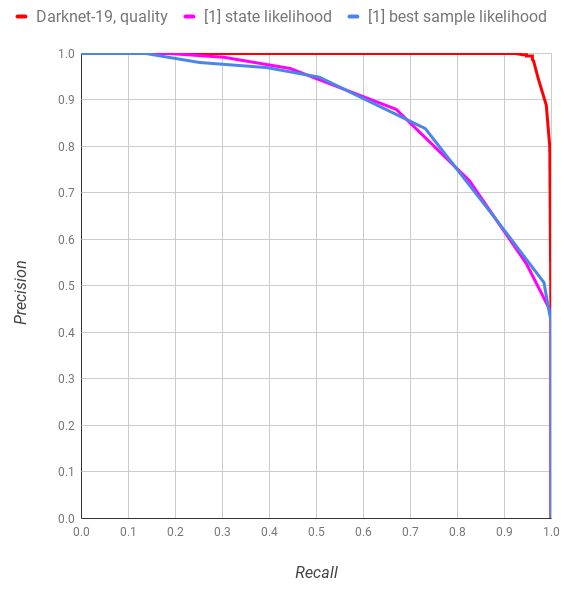
\includegraphics[width=0.8\columnwidth]{quality_net_PR_curve.png}}}
  \centering{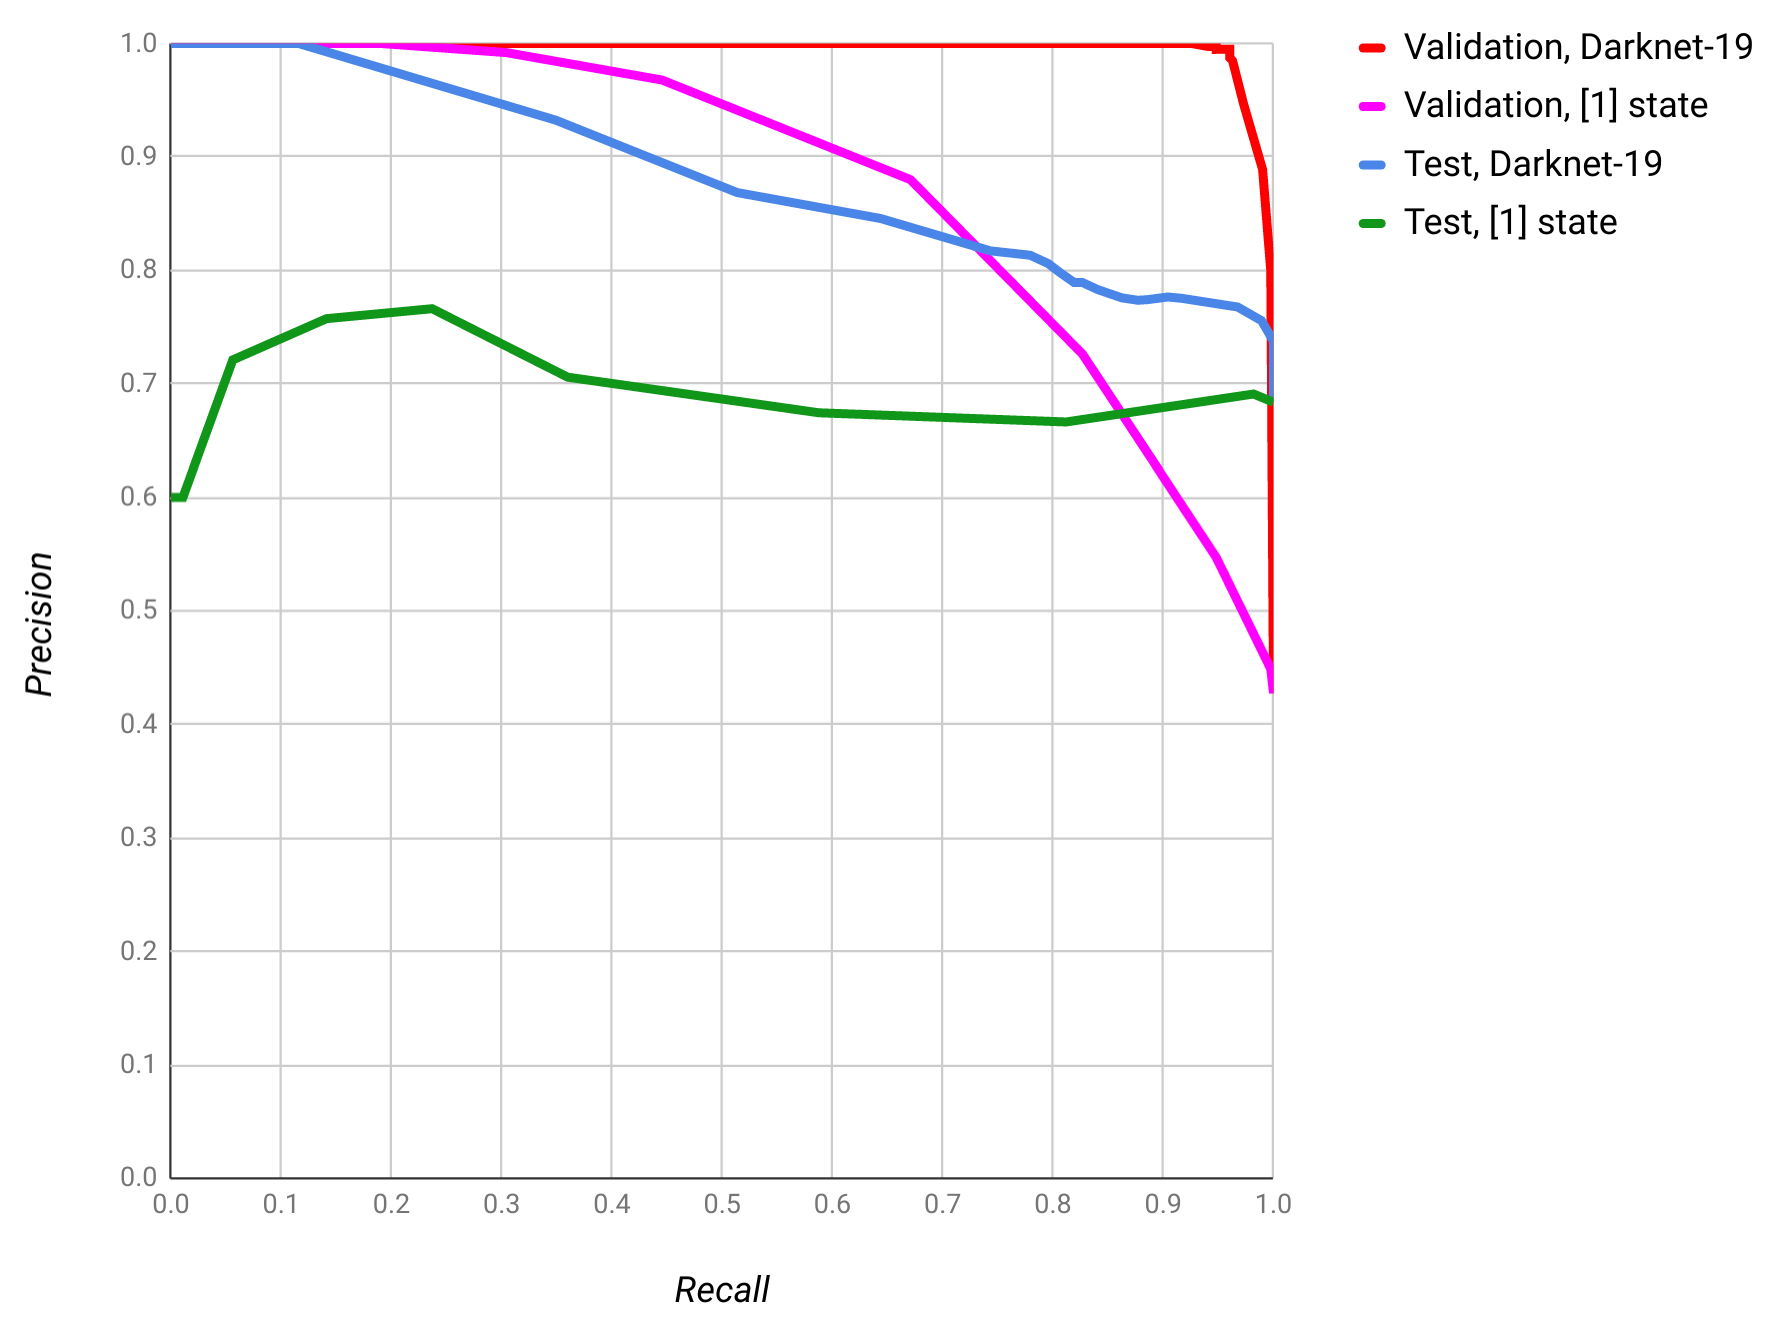
\includegraphics[width=1.0\columnwidth]{new_bad_trail_pr_curves.png}}}
\caption{Precision-recall curves on validation, test sets of different methods for assessing whether image contains a \textit{good} trail region or not.}
\label{fig:quality_results}
\end{figure}

%%%%%%%%%%%%%%%%%%%%%%%%%%%%%%%%%%%%%%%%%%%%%%%%%%%%%%%%%%%%%%%%%%%%%%%%%%%%%%%%

%%%%%%%%%%%%%%%%%%%%%%%%%%%%%%%%%%%%%%%%%%%%%%%%%%%%%%%%%%%%%%%%%%%%%%%%%%%%%%%%

\subsection{Trail segmentation}

% simplified VGG-16 = VGG-11 approach,

%blah blah convolutional front-end attached
%  through several fully-connected layers to an $(x, y, w, h)$ output
%  layer.}

The accuracy of any predicted trail quadrilateral was assessed by
computing the intersection over union (IoU) between it and the ground
truth quadrilateral, with IoUs $\geq 0.5$ considered ``correct''
segmentations.

The base training set of trail shape images was augmented by randomly
distorting both photometrically and geometrically
\comment{parameters?} each image $10\times$ yield a \textit{trail
  shape} training set of 16,140 images.  Any geometric distortion
which resulted in a particular trail becoming \textit{bad} was regenerated.

$\TrailOneDMaskNet$ was trained for 5000 iterations with a learning
rate of 0.0001 (batch size 128).  At test time, the output layer was
binarized with a threshold of 0.5 and a maximum gap of 3 to obtain the
trail quadrilateral vertices.  Note that for a few images this resulted in no
pixels on $\TrailFarLine$ having a value of 1, so $\hat{x}^{L}_{far}$
and $\hat{x}^{R}_{far}$ could not be inferred.  In these cases, an IoU
of 0 was assigned.

\cite{<FSR2012>}'s trail segmentation method outputs a polygon,
possibly curved, over a slightly larger depth range.  In order to
compute the IoU more fairly, the intersections of this polygon with
$\TrailFarLine$ and $\TrailNearLine$ are used to define the estimated
trail quadrilateral.  \comment{explanatory image?}

%%%%%%%%%%%%%%%%%%%%%%%%%%%%%%%%%%%%%%%%%%%%%%%%%%%%%%%%%%%%%%%%%%%%%%%%%%%%%%%%
\begin{table}
  \begin{center}
  \begin{tabular}{ |c|c c|c c| }
    \hline
    & \multicolumn{2}{|c|}{\textit{Validation}} & \multicolumn{2}{|c|}{\textit{Test}} \\
 %      & cell8 & cell9 & cell2 & cell3 \\ 
 %\hline
                        & \begin{tabular}{@{}c@{}}Median\\IoU\end{tabular} & \begin{tabular}{@{}c@{}}\%\\correct\end{tabular}  & \begin{tabular}{@{}c@{}}Median\\IoU\end{tabular} & \begin{tabular}{@{}c@{}}\%\\correct\end{tabular} \\
%   & Median IoU & \% correct & Median IoU & \% correct \\
 \hline
  $\TrailOneDMaskNet$    & \textbf{0.880} & 0.988          & \textbf{0.777} & \textbf{0.926} \\ 
  $\TrailRegressionNet$  & 0.835          & \textbf{0.993} & 0.738          & 0.902 \\ 
 \cite{<FSR2012>}        & 0.819          & 0.879          & 0.695          & 0.857 \\ 
 \hline
\end{tabular}
  \end{center}
  \caption{Trail segmentation results on images with shape annotations}
  \label{tab:shape_results}
  \end{table}
  
%%%%%%%%%%%%%%%%%%%%%%%%%%%%%%%%%%%%%%%%%%%%%%%%%%%%%%%%%%%%%%%%%%%%%%%%%%%%%%%%

Trail shape segmentation results are summarized in Tab.~\ref{tab:shape_results}.
  
\comment{say something about speed}

\comment{image gallery.  maybe columns are methods (including GT), rows are different images, some good, some bad from validation and test.  also thought about histogram of IoUs}

%\comment{performance of Darknet-19 trail segmentation after training.
%  Report mean SSD, pixel correctness?}

%$\TrailAnnotatedSet$ was divided into train/test with an 80/20 split:
%1,614 training images and 404 test images

\comment{class imbalance: 80\% of pixels are background, only 20\% are trail.  looked into this on september 28, 2016 -- weighting false negatives more than false positives in loss function did not help}

%\comment{trail masks have no confidence associated with them.  we can use output
%  of trail quality network for this.  need to compare to how
%  i got confidence in \cite{<FSR2012>}}

%%%%%%%%%%%%%%%%%%%%%%%%%%%%%%%%%%%%%%%%%%%%%%%%%%%%%%%%%%%%%%%%%%%%%%%%%%%%%%%%

\subsection{Trail tracking}

%%%%%%%%%%%%%%%%%%%%%%%%%%%%%%%%%%%%%%%%%%%%%%%%%%%%%%%%%%%%%%%%%%%%%%%%%%%%%%%%

\begin{figure}[!t]
\captionsetup[subfigure]{labelformat=empty}
\subfloat[]{%
  \centering{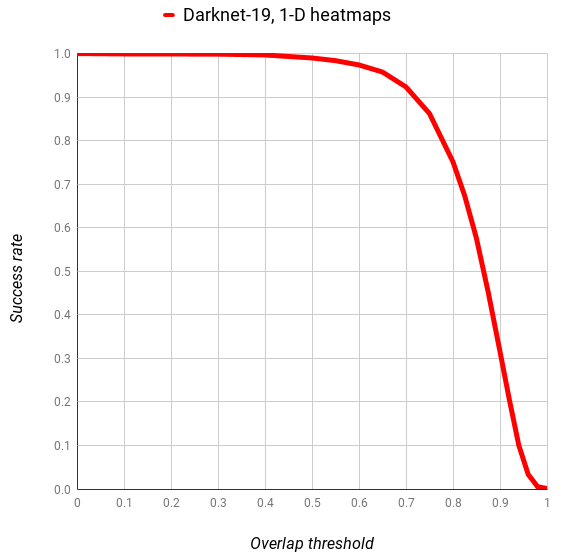
\includegraphics[width=0.8\columnwidth]{new_SP1_test.png}}}
\caption{Success plot of \comment{different} trail tracking methods on $\TrailSeqAnnotatedSet$ validation set.}
\label{fig:SP1_test}
\end{figure}

%%%%%%%%%%%%%%%%%%%%%%%%%%%%%%%%%%%%%%%%%%%%%%%%%%%%%%%%%%%%%%%%%%%%%%%%%%%%%%%%

\comment{what about that one in $\TrailSeqAnnotatedSet$ with the trail outside image in sequence?  it makes that training set 1,603.}

\comment{use standard tracking metric (AUC of success plot?) for both methods on test sequences}

\comment{some comparison to previous trail work? \cite{<GiustiTrail>} (data here: http://people.idsia.ch/~guzzi/DataSet.html) and/or \cite{<NvidiaTrail>}}

\comment{how is tracking performance measured over sequence?  In benchmark paper \cite{WuLimYang13}, these seem most relevant:}

%``Recently the precision plot [6, 27] has
%been adopted to measure the overall tracking performance.
%It shows the percentage of frames whose estimated location
%is within the given threshold distance of the ground truth.
%As the representative precision score for each tracker we
%use the score for the threshold = 20 pixels [6]''

%``Success plot.  Another evaluation metric is the bounding
%box overlap [IoU]...

\comment{``To measure the performance
on a sequence of frames, we count the number of
successful frames whose overlap S is larger than the given
threshold $t_{o}$. The success plot shows the ratios of successful
frames at the thresholds varied from 0 to 1. Using one
success rate value at a specific threshold (e.g. $t_{o}=0.5$) for
tracker evaluation may not be fair or representative. Instead
we use the area under curve (AUC) of each success plot to
rank the tracking algorithms.''}

\comment{``Robustness Evaluation. The conventional way to evaluate
trackers is to run them throughout a test sequence with initialization
from the ground truth position in the first frame
and report the average precision or success rate. We refer
this as one-pass evaluation (OPE). However a tracker
may be sensitive to the initialization, and its performance
with different initialization at a different start frame may
become much worse or better. Therefore, we propose two
ways to analyze a tracker’s robustness to initialization, by
perturbing the initialization temporally (i.e., start at different
frames) and spatially (i.e., start by different bounding
boxes).''}

\comment{From \cite{<VOT2016>}: ``Whenever a tracker
predicts a bounding box with zero overlap with the ground truth, a failure is
detected and the tracker is re-initialized five frames after the failure. Cehovin et ˇ
al. [20] identified two highly interpretable weakly correlated performance measures
to analyze tracking behavior in reset-based experiments: (i) accuracy and
(ii) robustness. The accuracy is the average overlap between the predicted and
ground truth bounding boxes during successful tracking periods. On the other
hand, the robustness measures how many times the tracker loses the target
(fails) during tracking.''}

%%%%%%%%%%%%%%%%%%%%%%%%%%%%%%%%%%%%%%%%%%%%%%%%%%%%%%%%%%%%%%%%%%%%%%%%%%%%%%%%

\subsection{Tree detection}

There are 127 images in $\TreeAnnotatedSet$ which belong to $\TrailAnnotatedSet$'s validation set.  These
contain 278 tree annotations.  \comment{this implies 523 images in $\TreeAnnotatedSet$ which belong to $\TrailAnnotatedSet$'s training set, containing 1162 annotated trees}

\comment{don't make YOLO ``learn'' the orientation of the trees.  we can predict orientation from
  position based on the omnidirectional calibration, or even from the annotation statistics.  why
  make the NN try to learn this?  thus, each tree BB only has 3 parameters: x, y of the bottom center, and
  the width}

\comment{in any gallery of anecdotal results, show trail region and detected trees together?}

% http://www.cv-foundation.org/openaccess/content_cvpr_2013/papers/Wu_Online_Object_Tracking_2013_CVPR_paper.pdf

%%%%%%%%%%%%%%%%%%%%%%%%%%%%%%%%%%%%%%%%%%%%%%%%%%%%%%%%%%%%%%%%%%%%%%%%%%%%%%%%
%%%%%%%%%%%%%%%%%%%%%%%%%%%%%%%%%%%%%%%%%%%%%%%%%%%%%%%%%%%%%%%%%%%%%%%%%%%%%%%%

\section{CONCLUSION}

\comment{restate what we did and its significance}

\comment{trail ROI and tree ROI don't use whole image for more efficient segmentation,
  yet still exhibit excellent performance}

\comment{next: run on real robot live.  feasible?  yes, because things run fast even on laptop}

\comment{utility of incorporating structure?}

The color/intensity contrast between the trail region and neighboring
regions depends heavily on the trail material and surrounding terrain
and vegetation. While it is sufficient in many situations, when the
contrast becomes too low trail tracking may deteriorate or fail
entirely. An additional cue which may compensate in these situations
is that of scene \textit{structure} along the trail, which may come
from a stereo depth map or ladar point cloud \cite{<FSR2012>}, a depth
camera such as a Kinect \cite{<KinectTrail>}, or structure-from-motion
\cite{<NvidiaTrail>}.

\comment{what would it mean to truly integrate the trail segmentation and the tree detection,
  rather than have them run independently?}

%%%%%%%%%%%%%%%%%%%%%%%%%%%%%%%%%%%%%%%%%%%%%%%%%%%%%%%%%%%%%%%%%%%%%%%%%%%%%%%%
%%%%%%%%%%%%%%%%%%%%%%%%%%%%%%%%%%%%%%%%%%%%%%%%%%%%%%%%%%%%%%%%%%%%%%%%%%%%%%%%

\addtolength{\textheight}{-12cm}   % This command serves to balance the column lengths
                                  % on the last page of the document manually. It shortens
                                  % the textheight of the last page by a suitable amount.
                                  % This command does not take effect until the next page
                                  % so it should come on the page before the last. Make
                                  % sure that you do not shorten the textheight too much.

%%%%%%%%%%%%%%%%%%%%%%%%%%%%%%%%%%%%%%%%%%%%%%%%%%%%%%%%%%%%%%%%%%%%%%%%%%%%%%%%
%%%%%%%%%%%%%%%%%%%%%%%%%%%%%%%%%%%%%%%%%%%%%%%%%%%%%%%%%%%%%%%%%%%%%%%%%%%%%%%%

\section*{ACKNOWLEDGMENTS}

\comment{NSF did pay for the robot, and the data used here was collected during the term of the CAREER.  Nvidia for graphics cards?}

%%%%%%%%%%%%%%%%%%%%%%%%%%%%%%%%%%%%%%%%%%%%%%%%%%%%%%%%%%%%%%%%%%%%%%%%%%%%%%%%
%%%%%%%%%%%%%%%%%%%%%%%%%%%%%%%%%%%%%%%%%%%%%%%%%%%%%%%%%%%%%%%%%%%%%%%%%%%%%%%%

{\small
\bibliographystyle{IEEEtran}
%\bibliographystyle{ieee}
\bibliography{trail_reference}
}

%\begin{thebibliography}{99}






%\end{thebibliography}




\end{document}
